\documentclass[12pt]{article}
\usepackage[utf8]{inputenc}
\usepackage[T1]{fontenc}
\usepackage[margin=0.45in]{geometry}
\usepackage{amsmath,amssymb}
\usepackage{booktabs}
\usepackage{graphicx}
\usepackage{enumitem}
\usepackage{makeidx}
\makeindex
\usepackage[hidelinks,bookmarksopen=true]{hyperref}
\usepackage{parskip}
\setlength{\parindent}{0pt}
\setlist{nosep,leftmargin=*}
% Number sections and subsections (e.g. 7, 7.1); subsubsections stay unnumbered
\setcounter{secnumdepth}{2}
\setcounter{tocdepth}{2}

\title{CSE 508 Network Security Cheat Sheet}
\author{Nikhil Shah}
\date{May 2026}

\begin{document}
\begin{titlepage}
\centering
{\LARGE\bfseries CSE 508 Network Security Cheat Sheet\par}
\vspace{1.5em}
{\large Nikhil Shah\par}
{\normalsize May 2026\par}
\vspace{1em}
{\normalsize Instructor: Omar Chowdhury\par}
\vspace{2em}
\hrulefill\par
\vspace{0.8em}
{\small
\begin{tabular}{c}
\textbf{Confidentiality}\index{confidentiality} --- Data is only accessible to authorized parties \\
\textbf{Integrity}\index{integrity} --- Data has not been tampered with or corrupted during transit \\
\textbf{Anonymity}\index{anonymity} --- Hide the identity of the participants of the communication
\end{tabular}
}
\par\vspace{0.8em}\hrulefill
\end{titlepage}

\renewcommand{\contentsname}{Table of Contents}
{\footnotesize\setlength{\parskip}{0.35ex}\tableofcontents}
\clearpage

\section{Study map and short practical notes}
\index{study map}

\subsection{CIA and related security goals}
\begin{itemize}
  \item \textbf{Confidentiality}\index{confidentiality}: data readable only by authorized parties.
  \item \textbf{Integrity}\index{integrity}: data not tampered with or corrupted in transit or storage.
  \item \textbf{Availability}\index{availability}: service remains usable; threatened by DoS/DDoS and operational failures (see Denial-of-Service).
  \item \textbf{Authentication}: verify who sent a message or owns a connection (certificates, MACs, signatures, pre-shared keys).
  \item \textbf{Anonymity / unlinkability}\index{anonymity}: hard to link actions or traffic to an identity (Tor, mixnets); encryption alone does not prevent traffic analysis.
\end{itemize}

\subsection{How this sheet is organized}
\begin{itemize}
  \item \textbf{Cryptography and trust (one block)}: Diffie--Hellman hardness; OTP and perfect secrecy; RSA; AES modes and AEAD; Merkle trees; MAC vs digital signatures; PKI (X.509); Certificate Transparency and ACME.
  \item \textbf{Common weaknesses}: static keys, missing randomness, weak hashing, plaintext handshakes (quick reference table).
  \item \textbf{Information flow, channels, privacy, DNS}: MLS-style labels, covert/side channels, CBC padding oracles, Tor and traffic analysis, DNS (incl.\ DNSSEC, CDN).
  \item \textbf{TLS and legacy application protocols}: TLS~1.3 record and handshake; FTP/FTPS/SFTP.
  \item \textbf{Denial of service}: volumetric, transport, application attacks and mitigations (incl.\ Smurf).
  \item \textbf{Perimeter, segmentation, and tunnels}: firewalls, VPNs, Zero Trust, L2/L3 boundaries, SSH tunneling.
  \item \textbf{Inter-domain routing}: BGP, eBGP/iBGP, hijacks/leaks, RPKI.
  \item \textbf{Lecture extras}: link-layer and Wi-Fi attacks (ARP, DHCP, CAM, deauth, evil packets).
\end{itemize}

\subsection{Symmetric vs asymmetric (when to use what)}
\begin{itemize}
  \item \textbf{Symmetric} (e.g.\ AES, ChaCha20): fast bulk encryption; requires a shared or derived session key.
  \item \textbf{Asymmetric} (RSA, DH/ECDH): key agreement or transport, signatures; expensive per operation --- usually establishes a symmetric key then records use symmetric crypto.
  \item \textbf{Hybrid (typical in TLS)}: certificates + signed handshake + ephemeral ECDHE for \textbf{forward secrecy}, then AEAD symmetric keys via HKDF.
\end{itemize}

\subsection{Integrity: MAC, signatures, and AEAD}
\begin{itemize}
  \item \textbf{MAC}: shared secret; integrity between parties who know the key; very fast; \textbf{no} non-repudiation.
  \item \textbf{Digital signature}: asymmetric; verifier needs only public key; \textbf{yes} non-repudiation (legal/code signing) via PKI.
  \item \textbf{AEAD} (AES-GCM, ChaCha20--Poly1305): confidentiality + integrity in one primitive; default for TLS records and new protocols.
  \item Prefer AEAD over ad hoc ``encrypt then MAC'' unless you follow a vetted composite construction; CBC+HMAC needs correct order and padding handling.
\end{itemize}

\subsection{Forward secrecy, randomness, and nonces}
\index{forward secrecy!practical notes}\index{randomness (cryptographic)}
\begin{itemize}
  \item \textbf{Forward secrecy (PFS)}: past sessions stay secret if long-term keys leak later; use \textbf{ephemeral} DH (ECDHE) in handshakes, not only static RSA key transport.
  \item \textbf{Randomness}: keys, IVs/nonces, and challenges must come from a CSPRNG; weak or predictable RNG breaks confidentiality and authentication.
  \item \textbf{Nonces / IVs}: for CTR and GCM, \textbf{never} reuse $(\text{key}, \text{nonce})$; reuse is catastrophic (keystream recovery, forgeries).
\end{itemize}

\subsection{Exam-style checklist}
\begin{itemize}
  \item \textbf{Speed vs non-repudiation}: MAC on the wire; signatures when origin must be provable to third parties.
  \item \textbf{IND-CPA}: deterministic public-key encryption (naive RSA) fails; use proper padding/hybrid schemes; OTP gives perfect secrecy only with ideal key management.
  \item \textbf{Network controls vs threat}: DNSSEC $\Rightarrow$ integrity/authentication of DNS data, not privacy (pair with DoH/DoT); RPKI $\Rightarrow$ origin validation for BGP prefixes, not full path attestation; WAFs and rate limits $\Rightarrow$ application-layer DoS.
\end{itemize}

\section{Diffie--Hellman}
\index{Diffie--Hellman}\index{DLP (discrete logarithm problem)}\index{CDH (computational Diffie--Hellman)}\index{DDH (decisional Diffie--Hellman)}
\begin{itemize}
  \item DLP (Discrete Logarithm Problem): given $g^a$, find $a$.
  \item CDH (Computational Diffie--Hellman): given $g^a$ and $g^b$, compute $g^{ab}$.
  \item DDH (Decisional Diffie--Hellman): given $g^a$, $g^b$ and a value $Z$, decide whether $Z=g^{ab}$ or $Z$ is random.
\end{itemize}

\hrulefill

\section{One--Time Pad (OTP)}
\index{one-time pad}\index{OTP|see{one-time pad}}\index{perfect secrecy}
\begin{itemize}
  \item Encrypt: ciphertext = plaintext XOR key (key length = message length).
  \item Perfect secrecy if: key is truly random, used only once, and kept secret.
  \item Danger: key reuse --- XOR of two ciphertexts cancels the key and leaks information.
\end{itemize}

\hrulefill

\section{RSA}
\index{RSA}\index{public-key encryption!RSA}\index{IND-CPA}
\begin{enumerate}[label=\arabic*.]
  \item \textbf{Key Generation}
    \begin{itemize}
      \item Select 2 primes $p$ and $q$
      \item $n = p \cdot q$
      \item select $d,e$ such that $x^{de} \bmod n = x$
      \item public key $\langle e,n\rangle$
      \item private key $\langle d,n\rangle$
    \end{itemize}
  \item \textbf{Encrypt using public key} --- $c = m^e \bmod n$
  \item \textbf{Decrypt with private key} --- $m = c^d \bmod n$
    \begin{itemize}
      \item RSA will be broken with Quantum Computing
      \item RSA is deterministic, so it fails IND-CPA
      \begin{itemize}
        \item Repeat of $M$ gets the exact same $C$
      \end{itemize}
    \end{itemize}
\end{enumerate}

\hrulefill

\section{AES Modes}
\index{AES}\index{block cipher modes}\index{ECB mode}\index{CBC mode}\index{CTR mode}\index{GCM}\index{CCM}\index{AEAD}\index{ChaCha20-Poly1305}
\begin{itemize}
  \item \textbf{AES-ECB --- Electronic Code Book}: Encrypts each 128-bit block independently ($C_i = E_K(P_i)$). Deterministic (same plaintext $\to$ same ciphertext), so it leaks patterns; avoid for multi-block data.
  \item \textbf{AES-CBC --- Cipher Block Chaining}: Uses a fresh random IV; encryption $C_i = E_K(M_i \oplus C_{i-1})$, decryption $M_i = C_{i-1} \oplus D_K(C_i)$. Provides chaining but needs integrity (MAC/AEAD) and correct IV handling to be secure.
  \item \textbf{AES-CTR --- Counter Mode}: Turns block cipher into a stream cipher using $E_K(\text{IV} + i)$; $C_i = M_i \oplus E_K(\text{IV}+i)$. Allows random access and efficient parallelism; nonce/IV must never repeat for a key.
  \item \textbf{AES-GCM/CCM (AEAD) --- Authenticated Encryption}: GCM (Galois/Counter) and CCM combine CTR-like encryption with an authentication tag (AEAD). Provide confidentiality + integrity in one primitive and are the recommended modes (used in TLS).
\end{itemize}

\begin{quote}
Use authenticated encryption (AEAD) whenever possible (e.g., GCM, ChaCha20--Poly1305).
\end{quote}

\hrulefill

\section{Merkle Tree (construction)}
\index{Merkle tree}\index{Merkle root|see{Merkle tree}}
\begin{enumerate}[label=\arabic*.]
  \item Hash each data block to produce leaves: $H_1, H_2, \ldots$.
  \item Pair neighboring leaves, concatenate pairs, and hash pairs to form parent nodes: e.g.\ $H_{12} = H( H_1 \Vert H_2 )$
  \item Repeat upward until a single root hash remains --- the Merkle root.
\end{enumerate}

\hrulefill

\section{MAC vs Digital Signature}
\index{message authentication code}\index{MAC|see{message authentication code}}\index{digital signature}\index{non-repudiation}
\begin{center}
\begin{tabular}{@{}lcc@{}}
\toprule
\textbf{Feature} & \textbf{MAC} & \textbf{Digital Signature} \\
\midrule
Key type & Symmetric (shared secret) & Asymmetric (public/private pair) \\
Speed & Very fast & Slower (public-key ops) \\
Non-repudiation & No & Yes \\
Primary use & Packet/message integrity & Legal docs, code signing, non-repudiation \\
\bottomrule
\end{tabular}
\end{center}

\hrulefill

\section{Public Key Infrastructure (PKI)}
\index{PKI}\index{X509@X.509}\index{certificate authority}\index{CSR (certificate signing request)}\index{CRL (certificate revocation list)}\index{HSM (hardware security module)}
\begin{itemize}
  \item Purpose: bind public keys to identities using certificates (X.509). CAs issue and sign certs; trust is anchored in root CA public keys.
  \item CA hierarchy: Root CA (trust anchor) $\to$ Intermediate CA(s) $\to$ End-entity certs; validation builds a chain to a trusted root.
  \item Certificate essentials: Subject, SubjectAltName (SAN), Issuer, Validity (notBefore/notAfter), Public Key, Signature, Extensions (keyUsage, EKU, basicConstraints, CRL/OCSP endpoints).
  \item Issuance flow: generate keypair + CSR (keep private key secret) $\to$ CA verifies identity $\to$ CA issues cert. Protect CA/keys (HSMs, secure ops).
  \item Revocation \& checking: CRLs (pull), OCSP (real-time), OCSP stapling (server-provided proof) --- clients must check expiry and revocation where required.
  \item Validation checklist: chain signature verification, expiry, CN/SAN name match, keyUsage/EKU policy, and revocation status.
  \item Threats \& mitigations: misissued or compromised CA $\to$ use Certificate Transparency (CT) logs, short-lived certs, strict auditing, key protection (HSM), and rapid revocation/patching.
  \item Ops note: automate issuance (ACME) + short lifetimes; enable OCSP stapling and monitor CT and revocation telemetry.
\end{itemize}

\hrulefill

\section{Certificate Transparency (CT) \& ACME}
\index{Certificate Transparency}\index{ACME}\index{SCT (signed certificate timestamp)}\index{Let's Encrypt|see{ACME}}\index{certificate misissuance}
\begin{itemize}
  \item Certificate Transparency: public, append-only logs of issued certificates. CAs submit certs to CT logs and return Signed Certificate Timestamps (SCTs).
    \begin{itemize}
      \item CT is a bulletin board for what CA issued what certificate. Needs to be confirmable. It is a deterrent to stop bad CAs.
      \item Initially get a Signed Certificate Timestamp with max merge of 24 hrs.
      \item Inclusion proof: see figure below; checks if your cert is inside the Merkle tree.
      \item SCTs are embedded in certificates or stapled by servers; monitors/auditors watch logs to detect misissuance.
      \item CT helps detect rogue or misissued certificates quickly by providing public visibility.
    \end{itemize}
\end{itemize}

\begin{center}
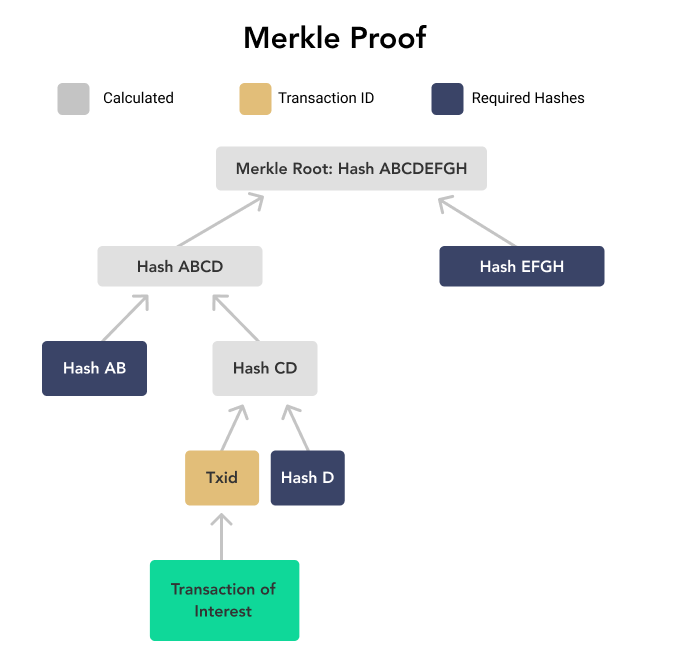
\includegraphics[width=0.75\linewidth]{media/MerkleProof.png}
\end{center}

\begin{itemize}
  \item ACME (Automated Certificate Management Environment): protocol (used by Let's Encrypt) for automated issuance/renewal of certificates.
    \begin{itemize}
      \item ACME uses challenges (HTTP-01, DNS-01, TLS-ALPN-01) to prove domain control and an account key for the requester.
      \item ACME + short-lived certs encourage automation and reduce manual CA processes.
      \item ACME --- Let's Encrypt is an automated way to provide free certs. But each cert is a short time. Needs to validate that you control the server and domain if you want a cert. No \texttt{*.domain.com} certs (wildcard note per original).
    \end{itemize}
  \item Overall ACME Protocol Flow
    \begin{enumerate}[label=\arabic*.]
      \item Client generates an account key pair and registers with the ACME server
      \item Client submits an order for a domain (e.g.\ \texttt{example.com})
      \item Server responds with an authorization object containing challenge options
      \item Client fulfils a challenge (HTTP-01 or DNS-01) and signals readiness
      \item Server verifies the challenge --- authorization marked valid
      \item Client submits a CSR signed with the domain key; server issues the certificate
    \end{enumerate}
\end{itemize}

\subsection{ACME Challenge Comparison (HTTP vs DNS)}
\index{HTTP-01 challenge}\index{DNS-01 challenge}\index{wildcard certificates}
\begin{center}
\begin{tabular}{@{}p{0.18\linewidth}p{0.38\linewidth}p{0.38\linewidth}@{}}
\toprule
\textbf{Challenge} & \textbf{Pros} & \textbf{Cons} \\
\midrule
\textbf{HTTP-01} & Easy to automate; doesn't require DNS API access; works on standard port 80. & \textbf{No wildcard support}; requires web server to be reachable on port 80; firewall must allow inbound traffic. \\
\textbf{DNS-01} & \textbf{Supports Wildcard certificates}; works for internal/private servers; no inbound port 80/443 required. & Requires automated API access to DNS provider (security risk); DNS propagation delays; complex setup. \\
\bottomrule
\end{tabular}
\end{center}

\hrulefill

\section{Common Weaknesses}
\index{forward secrecy}\index{perfect forward secrecy|see{forward secrecy}}\index{replay attacks}\index{SHA-256}\index{nonces}
\begin{center}
\begin{tabular}{@{}p{0.22\linewidth}p{0.32\linewidth}p{0.38\linewidth}@{}}
\toprule
\textbf{Weakness} & \textbf{Typical attack} & \textbf{Mitigation} \\
\midrule
Static keys & Retrospective decryption & Use ephemeral keys (Perfect Forward Secrecy) \\
No randoms & Replay attacks & Use nonces, sequence numbers, timestamps \\
Weak hashing & Collision attacks & Use SHA-256 or stronger \\
Plaintext handshake & Eavesdropping & Encrypt handshake (modern TLS) \\
\bottomrule
\end{tabular}
\end{center}

\hrulefill

\section{Information Flow \& Side--Channels}
\index{information flow}\index{side-channel attacks}\index{covert channels}\index{noninterference}\index{constant-time implementations}
\begin{itemize}
  \item Information Flow (MLS concepts): reason about how data labeled \texttt{High} (secret) may influence \texttt{Low} (public) outputs; properties: noninterference (no flow from High$\to$Low) and non-deducibility (observer cannot eliminate high inputs).
  \item Covert channels: unintended channels (timing, resource usage, stdout) that leak high data through low-observable behavior; examples: timing delays, process scheduling, file system metadata.
  \item Side-channel attacks: timing, cache, power, electromagnetic analysis; attackers exploit observable differences in implementations to recover secrets.
  \item Defenses: constant-time implementations, noise/padding, reduce observable state, limit precision of timers, blinding (RSA), algorithmic changes and rate-limiting of error messages.
\end{itemize}

\subsection{CBC Padding Oracle (Vaudenay / Lucky13)}
\index{padding oracle}\index{Vaudenay attack}\index{Lucky13}\index{PKCS7@PKCS \#7 padding}\index{encrypt-then-MAC}
\begin{itemize}
  \item Background: PKCS\#7 padding adds $p$ bytes each with value $p$; invalid padding triggers errors that may be observable to an attacker.
  \item Vaudenay padding oracle: adaptive chosen-ciphertext attack that uses padding validity responses to decrypt CBC ciphertexts without the key by manipulating ciphertext blocks.
  \item Lucky13 (TLS/DTLS): timing side-channel from MAC+padding processing that leaks information about padding length; exploits subtle timing differences in record processing.
  \item Mitigations: use AEAD modes (GCM/CCM) or encrypt-then-MAC constructions; ensure indistinguishable error handling (uniform error messages and constant-time processing); avoid returning padding validity to callers; apply strict record parsing and constant-time MAC checks.
\end{itemize}

\subsection{Privacy, Anonymity \& Tor}
\index{privacy}\index{Tor}\index{onion routing}\index{mixnets}\index{traffic analysis}\index{fingerprinting (browser)}\index{hidden services (Tor)}
\begin{itemize}
  \item Privacy vs Anonymity: privacy controls collection/use of PII; anonymity prevents linking actions to identities (unlinkability). Pseudonymity provides persistent but unlinkable identifiers.
  \item Threat models: local observers (ISP), on-path adversaries, endpoint collusion, global passive observers; always assume some intermediaries may be adversarial --- TLS alone does not solve traffic analysis.
  \item Fingerprinting \& traffic analysis: browser/device fingerprinting (canvas, WebGL, fonts, AudioContext, battery), and website fingerprinting (packet sizes/timing) can deanonymize users even over encrypted channels.
  \item Anonymity sets \& mixnets: larger anonymity sets increase unlinkability; mixers (mixnets) add batching and reordering to defeat timing correlation at the cost of latency and throughput.
  \item Tor highlights: onion routing with entry guards, middle relays, exit nodes; client builds layered encryption (three-hop circuits), resists single-relay compromise but is vulnerable to global passive adversaries and website fingerprinting.
  \item Hidden services: use introduction points, rendezvous points, and service descriptors (DHT) to publish and connect without exposing IPs; operational care needed to avoid deanonymizing metadata.
  \item Defenses/operational tips: reduce fingerprinting surface (resist JS fingerprinting, use Tor Browser), prefer high-latency mixnets for strong anonymity when acceptable, pad and shape traffic (where feasible), monitor ingress/egress correlation risks, use entry guards and avoid reusing circuits for sensitive links.
\end{itemize}

\subsection{DNS Protocol Recap}
\index{DNS}\index{DNS cache poisoning}\index{DNS amplification}\index{EDNS(0)}\index{AXFR}\index{TSIG}
\begin{itemize}
  \item Flow: stub resolver $\to$ recursive resolver $\to$ root $\to$ TLD $\to$ authoritative server; resolver caches and returns the answer.
  \item Transport: UDP/53 (default, fast); TCP/53 (truncation, large responses, AXFR); DoT/DoH for encrypted queries.
  \item Key fields \& RRs (very quick): 16-bit TXID; flags (QR, TC, RD, RA); counts (QD/AN/NS/AR); common RRs: A, AAAA, NS, CNAME, MX, PTR, TXT, SOA.
  \item Caching/TTL: answers cached for TTL seconds; negative caching via SOA; TTL controls propagation/staleness window.
  \item Important extensions: EDNS(0) (larger UDP payloads), DNS Cookies, QNAME minimization.
  \item Attacks \& short mitigations: cache poisoning $\to$ TXID+source-port randomization + DNSSEC; amplification $\to$ close/harden open resolvers + rate-limit; on-path tampering $\to$ DoT/DoH.
  \item Ops notes: TC$\to$retry over TCP; restrict/authenticate AXFR (TSIG); avoid open recursive resolvers.
\end{itemize}

\begin{center}
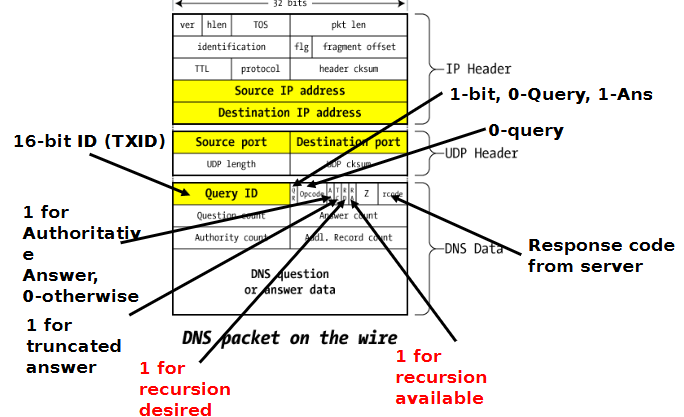
\includegraphics[width=0.85\linewidth]{media/DNSPacket.png}
\end{center}

\subsubsection{DNSSEC}
\index{DNSSEC}\index{chain of trust!DNS}
\begin{itemize}
  \item Adds digital signatures to DNS records and a chain of trust (root $\to$ TLD $\to$ authoritative).
  \item Provides integrity and authentication, but not privacy (DNSSEC responses are still visible unless combined with DoT/DoH).
\end{itemize}

\subsubsection{CDN (Content Delivery Network) \& DNS}
\index{CDN (content delivery network)}\index{EDNS client subnet}
\begin{itemize}
  \item CDNs use DNS (geo-DNS / EDNS client subnet) or HTTP redirects to point clients to a nearby PoP (edge server) IP.
  \item Flow: resolver $\to$ authoritative CDN DNS $\to$ returns IP for best PoP (may use client IP or ECS); TTLs are kept short for agility.
  \item Benefits: caches content closer to users, reduces origin load, improves latency, and absorbs volumetric DDoS traffic at edges.
  \item Risks: DNS compromise or cache poisoning can redirect users; low TTLs increase DNS query load; EDNS client subnet leaks partial client location to CDNs.
  \item Mitigations: protect authoritative DNS (DNSSEC, Anycast, rate-limit), use CDN security features (WAF, DDoS mitigation), monitor edge health and origin failover.
\end{itemize}

\hrulefill

\section{SSL/TLS}
\index{TLS}\index{SSL|see{TLS}}\index{TLS 1.3|see{TLS}}\index{ECDHE}\index{HKDF}\index{OCSP}\index{OCSP stapling}\index{SNI}\index{PSK (pre-shared key)}\index{HTTPS}
\begin{itemize}
  \item Purpose: provides encryption (confidentiality), integrity, and server/client authentication for application protocols (e.g., HTTPS, IMAPS).
  \item TLS 1.3 (modern) handshake, high level:
    \begin{itemize}
      \item ClientHello (versions, cipher suites, key\_share, SNI, PSK offers) $\to$ ServerHello (chosen suite, server key\_share).
      \item Encrypted handshake: EncryptedExtensions, Certificate, CertificateVerify, Finished --- most handshake data after ServerHello is encrypted.
      \item Key exchange: ECDHE (ephemeral) for forward secrecy; symmetric keys derived with HKDF.
      \item Record layer: AEAD ciphers (e.g., AES-GCM, ChaCha20-Poly1305) provide combined auth+enc.
    \end{itemize}
  \item Key features: authenticated encryption (AEAD), ephemeral key exchange (ECDHE), session resumption via PSK/tickets, optional 0-RTT early data (replay risks).
  \item Certificate validation: verify chain, check CN/SAN, validity window, revocation methods (OCSP/CRL/OCSP stapling); TLS session resumption relies on ticket/PSK trust.
  \item Operational notes: prefer TLS 1.3; disable legacy cipher suites and renegotiation; enable OCSP stapling and short-lived certs where possible.
\end{itemize}

\subsection{TLS 1.3 Protocol Exchange (1-RTT overview)}
\index{TLS 1.3!handshake}\index{ClientHello}\index{Finished message (TLS)}
\begin{enumerate}[label=\arabic*.]
  \item \textbf{ClientHello} --- client sends supported cipher suites and a KeyShare (e.g., ECDHE public key share).
  \item \textbf{ServerHello \& Response} --- server replies with selected cipher suite, server KeyShare; sends encrypted extensions and Certificate; includes Finished MAC to prove handshake integrity.
  \item \textbf{Client Finished} --- client verifies server Certificate and Finished; sends its own Finished message.
\end{enumerate}
TLS 1.3 reduces round trips by sending key shares early; handshake keys derive from ECDHE and certificates.

\subsection{TLS --- Common vulnerabilities \& pitfalls}
\index{Heartbleed}\index{downgrade attacks}\index{0-RTT}\index{certificate validation}
\begin{itemize}
  \item Certificate issues: misissued or compromised CAs, improper chain/hostname/expiry checks, and unreliable revocation handling (CRL/OCSP).
  \item Protocol downgrade \& legacy ciphers: fallback to weak suites enables downgrade attacks.
  \item Handshake/implementation bugs: e.g., Early CCS and similar flaws that allow weak keying or transcript manipulation.
  \item 0-RTT replay risks: TLS 1.3 early data may be replayed unless mitigated at the application layer.
  \item RNG \& key management: poor randomness, nonce reuse, and long-lived keys (no PFS) weaken security.
  \item Side-channel and memory bugs: timing/oracle attacks, Heartbleed-style memory leaks, and other implementation defects.
\end{itemize}

\section{FTP (File Transfer Protocol)}
\index{FTP}\index{FTPS}\index{SFTP}\index{PASV mode}\index{PORT mode (FTP)}
\begin{itemize}
  \item Plaintext protocol: control channel (TCP/21) sends commands and credentials in cleartext by default.
  \item Active vs Passive modes:
    \begin{itemize}
      \item Active (PORT): client opens ephemeral port, tells server to connect back $\to$ NAT/firewall issues because server connects to client.
      \item Passive (PASV): server opens ephemeral data port, client connects $\to$ better for clients behind NAT.
    \end{itemize}
  \item Security: use \texttt{FTPS} (FTP over TLS) or \texttt{SFTP} (SSH File Transfer, different protocol) instead of plain FTP.
  \item Common mitigations: disable anonymous access, require strong auth, limit and firewall data port ranges (and document them), prefer SFTP/FTPS, log transfers, chroot or restrict user directories.
\end{itemize}

\hrulefill

\section{Denial-of-Service (DoS)}
\index{denial of service}\index{DDoS|see{denial of service}}\index{SYN flooding}\index{SYN cookies}\index{Slowloris}\index{HTTP/2 Rapid Reset}\index{amplification attacks}
\begin{itemize}
  \item Goal: deny or degrade availability. Often distributed (DDoS); can exhaust bandwidth, CPU, memory, sockets, or human attention.
  \item Categories:
    \begin{itemize}
      \item Volumetric / Amplification: spoofed small requests cause much larger replies (Smurf, DNS/NTP/CLDAP/SSDP).
      \item Transport/state exhaustion: SYN flooding (half-open connections), TCP RST injection to kill sessions.
      \item Application-layer: connection flooding, Slowloris, HTTP/2 Rapid Reset, and algorithmic complexity attacks.
    \end{itemize}
  \item Short mitigations:
    \begin{itemize}
      \item Network: upstream filtering, ingress/egress filtering (uRPF), Anycast/CDN, blackholing and capacity planning.
      \item Transport: SYN cookies, drop old half-opens, connection limits, TCP timeouts, rate limiting.
      \item Application: WAFs, request rate-limits, resource quotas, fix algorithmic worst-cases (input validation, safer parsers).
      \item Amplification-specific: disable/respond-to-broadcasts, restrict/harden open UDP services, close open resolvers, apply rate limits.
    \end{itemize}
  \item Extra notes: Smurf (broadcast amplification), SYN cookies (stateless SYN defense), Slowloris (hold connections open), HTTP/2 Rapid Reset (stream-reset abuse).
\end{itemize}

\subsection{Smurf Attacks}
\index{Smurf attack}\index{ICMP amplification|see{Smurf attack}}
\begin{itemize}
  \item Mechanism: attacker spoofs victim IP as source and sends ICMP Echo requests to a broadcast address; many hosts reply to the victim causing amplification.
  \item Requirements: networks that respond to directed/broadcast pings and lack ingress filtering for spoofed IPs.
  \item Mitigations: disable IP-directed broadcasts on routers, configure hosts to ignore broadcast ICMP, apply ingress filtering/uRPF to block spoofed source IPs, and block/ratelimit ICMP from untrusted sources.
\end{itemize}

\hrulefill

\section{Firewalls \& Tunnels}
\index{firewall}\index{access control list}\index{stateful firewall}\index{NGFW}\index{UPnP}\index{VPN}\index{IPsec@IPsec}\index{OpenVPN}\index{WireGuard}\index{NAT traversal}\index{STUN/TURN}
\begin{itemize}
  \item Firewalls:
    \begin{itemize}
      \item Types: stateless (ACLs), stateful (tracks sessions), NGFW (L7 inspection).
      \item Rule order (quick): \texttt{allow RELATED,ESTABLISHED} $\to$ allow required services $\to$ \texttt{default-deny}.
      \item Placement: edge chokepoint + internal segmentation (VLAN/DMZ).
      \item Pitfalls: open management ports, UPnP/auto-port-mapping, misordered rules, broad CIDRs.
      \item UPnP (auto port-mapping) --- brief: allows LAN apps to request NAT/firewall port openings dynamically (automatic port forwarding).
        \begin{itemize}
          \item Why it's a flaw: typically unauthenticated and enabled by default on consumer gateways so malware or malicious apps can open WAN-accessible ports, exposing internal services.
          \item Mitigations: disable UPnP on edge devices unless necessary, use explicit/manual port forwarding, restrict UPnP to trusted LAN interfaces, keep firmware patched, and monitor/clear dynamic mappings; block IGD/UPnP traffic on the WAN side.
        \end{itemize}
      \item Each rule is priority top to bottom:
        \begin{itemize}
          \item $\langle\text{sourceIP}, \text{sourcePort}, \text{destinationIP}, \text{destinationPort}, \text{condition}, \text{protocol}, \text{decision}\rangle$
          \item $\langle\text{localhost}, *, X, 22, *, \text{SSH/TCP}, \text{allow}\rangle$ --- allow outgoing ssh connections
          \item $\langle*, *, *, *, \text{true}, *, \text{deny}\rangle$ --- default-deny rule outline
        \end{itemize}
    \end{itemize}
  \item Tunnels / VPNs:
    \begin{itemize}
      \item Use SSH Tunneling to bypass a restrictive firewall by allowing tcp forwarding and port translating to allow web surfing from the server's visibility
      \item IPSec (site-to-site, transport vs tunnel mode), OpenVPN/TLS-based VPNs, WireGuard (modern, simple, fast), SSH tunnels.
      \item Use strong auth (certificates or strong PSKs), encrypt both control and data planes, and enable perfect forward secrecy where possible.
      \item NAT traversal: NAT-T for IPsec, UDP encapsulation, STUN/TURN for P2P apps.
    \end{itemize}
\end{itemize}

\subsection{Zero Trust (brief)}
\index{zero trust}\index{microsegmentation}
\begin{itemize}
  \item Principle: ``Never trust, always verify'' --- authenticate \& authorize every access request regardless of network location.
  \item Key controls: identity \& device posture checks, least privilege, microsegmentation (per-service policies), continuous logging/telemetry and conditional access policies.
  \item Why use it: reduces lateral movement and blast radius compared with flat trust models; enforce via IAM, device management, service mesh, or policy engines.
\end{itemize}

\subsection{L2 vs L3 boundaries (network segmentation)}
\index{VLAN}\index{network segmentation}\index{Dynamic ARP Inspection|see{ARP spoofing}}
\begin{itemize}
  \item L2 (layer 2): switches, MAC forwarding, VLANs --- good for local segmentation but susceptible to ARP spoofing, CAM table floods, and broadcast storms; use port-security and DAI at access layer.
  \item L3 (layer 3): routers/firewalls, IP routing and ACLs --- enforces routing boundaries and IP-level filtering, reduces broadcast domains and offers clearer policy enforcement for inter-VLAN traffic.
  \item Design note: combine both --- use L2 isolation (VLANs) at access, enforce inter-VLAN policies at L3 (firewall/router), and apply microsegmentation for sensitive workloads.
\end{itemize}

\subsection{SSH Tunneling --- what it is and how it bypasses firewalls}
\index{SSH tunneling}\index{bastion host}\index{port forwarding!SSH}
\begin{itemize}
  \item What it is: SSH tunneling uses an authenticated, encrypted SSH connection as a generic transport to carry other TCP connections or proxy traffic through a permitted channel. The SSH connection acts as an encrypted pipe between the client and an SSH server (often a bastion or jump host).
  \item How it bypasses firewalls: many networks allow outbound SSH (or another allowed port) to reach an internal/edge host. By encapsulating application traffic inside the SSH session, clients can send and receive data to/through the SSH server even when direct connections are blocked by firewall rules. The SSH server then forwards the encapsulated traffic to the final destination from its network perspective, so the firewall only sees an allowed SSH session rather than the blocked application-level flows.
  \item Common uses (conceptually): local forwarding (forward a remote service to a local port), remote forwarding (expose a local service via the server's network), and dynamic proxying (tunnel multiple connections through the SSH channel). These are types of forwarding behavior rather than new protocols.
  \item Security implications: the SSH endpoint becomes an exit point --- outgoing traffic from the server's network may be visible to that host, and misuse can expose internal services. Authentication should be strong (keys, not passwords), server-side restrictions should be applied (limit permitted forwards and bind addresses), and monitoring/logging of forwarded connections is recommended.
\end{itemize}

\hrulefill

\section{BGP (Border Gateway Protocol)}
\index{BGP}\index{autonomous system}\index{AS path@AS\_PATH}\index{RPKI}\index{ROA (route origin authorization)}\index{route hijacking}\index{BGPmon}
\begin{itemize}
  \item Purpose: inter-domain routing between Autonomous Systems (ASes). BGP runs over TCP port 179 and exchanges route announcements (prefixes + attributes).
  \item Core message types: OPEN, UPDATE (announcements/withdrawals), KEEPALIVE, NOTIFICATION.
  \item Route selection (simplified): highest local-pref $\to$ shortest AS\_PATH $\to$ lowest origin type $\to$ lowest MED $\to$ eBGP over iBGP $\to$ lowest IGP cost to next-hop.
  \item Common issues: route hijacks (malicious or accidental announcements), prefix leaks, AS path manipulation.
  \item Mitigations: prefix filtering and route-policy, max-prefix limits, IRR-based filtering, RPKI/ROA origin validation (detect bogus origin AS), monitoring (BGPmon), and strict peering policies.
\end{itemize}

\subsection{eBGP vs iBGP}
\index{eBGP}\index{iBGP}\index{route reflector}
\begin{itemize}
  \item eBGP (external BGP): runs between different Autonomous Systems (ASes). Peers are typically directly connected; eBGP updates normally modify the \texttt{AS\_PATH} (prepend local AS) and are used to advertise reachability to the global Internet.
  \item iBGP (internal BGP): runs within a single AS. iBGP preserves \texttt{AS\_PATH} (does not prepend) and peers may be multiple hops away; routes learned from one iBGP peer are not re-advertised to another iBGP peer (split-horizon), so a full mesh or route reflectors are required for scalability.
  \item Operational notes: eBGP sessions often assume adjacent peers and may use TTL/adjacency checks; iBGP requires careful topology (full mesh, route reflectors, or confederations) to ensure route propagation and avoid loops.
\end{itemize}

\subsection{BGP --- Security risks}
\index{BGP!security risks}\index{prefix leak}\index{route leak|see{prefix leak}}
\begin{itemize}
  \item Prefix hijacking: an AS advertises IP prefixes it does not own (maliciously or by misconfiguration), causing traffic to be diverted or dropped.
  \item Route leaks: an AS improperly advertises routes learned from one peer to others, exposing prefixes to unintended paths and disrupting routing.
  \item Path manipulation \& AS\_PATH spoofing: altering \texttt{AS\_PATH} or prepending to influence route selection and route acceptance.
  \item Lack of authentication: classic BGP has no cryptographic origin/path validation, enabling impersonation and false announcements.
  \item Session attacks: TCP-level attacks (RST injection, session hijacking) or compromised peers can inject malicious UPDATEs.
  \item Instability \& amplification: frequent bogus announcements/withdrawals (flapping) can create routing instability and large control-plane loads.
  \item RPKI/ROA risks \& operational pitfalls: incomplete deployment, misconfigured ROAs, and reliance on a centralized trust infrastructure can cause accidental outages or false validation failures.
  \item Impact: traffic interception (MitM), blackholing, censorship, interception for data exfiltration or DDoS amplification via misdirected traffic.
\end{itemize}

\textit{(Note from source: lower content amount)}

\textbf{Brief mitigations:} strict prefix filtering, IRR/RPKI origin validation, max-prefix and sanity checks, neighbor authentication/ACLs, TTL/adjacency protections, monitoring and rapid remediation (BGPmon, route collectors).

\hrulefill

\section{Lecture extras}
\index{ARP spoofing}\index{DHCP snooping}\index{CAM table flooding}\index{evil twin attack}\index{802.11w}\index{Ping of Death@Ping-of-Death}
\begin{itemize}
  \item ARP poisoning / spoofing: inject fake ARP replies to poison host caches (enables MITM); defend with static bindings, Dynamic ARP Inspection (DAI) and monitoring.
  \item DHCP exhaustion / rogue DHCP: consume IP pool or run fake servers to disrupt clients; mitigate with DHCP snooping, trusted switch ports and rate limits.
  \item MAC/CAM table flooding: flood switches with fake MACs to overflow the CAM table and force fail-open behavior; use port security and MAC limits.
  \item Wi-Fi deauth \& evil-twin: send spoofed deauth frames or run rogue APs to disconnect or capture clients; mitigate with 802.11w (MFP), WPA2/3 and strong AP authentication.
  \item ``Evil packet'' exploits (Ping-of-Death, LAND, Teardrop): crafted packets that trigger kernel/stack bugs and crashes; defend by patching, ingress filtering, and fragmentation checks.
  \item Operational defenses (lecture): enable DHCP snooping/DAI on switches, disable IP-directed broadcasts (Smurf mitigation), restrict open resolvers and close unnecessary UDP services.
\end{itemize}

\clearpage
\phantomsection
\addcontentsline{toc}{section}{Index}
\printindex

\end{document}
